%!TEX root = root.tex

\begin{vita}

\begin{wrapfigure}{r}{0.3\textwidth}
    \centering
    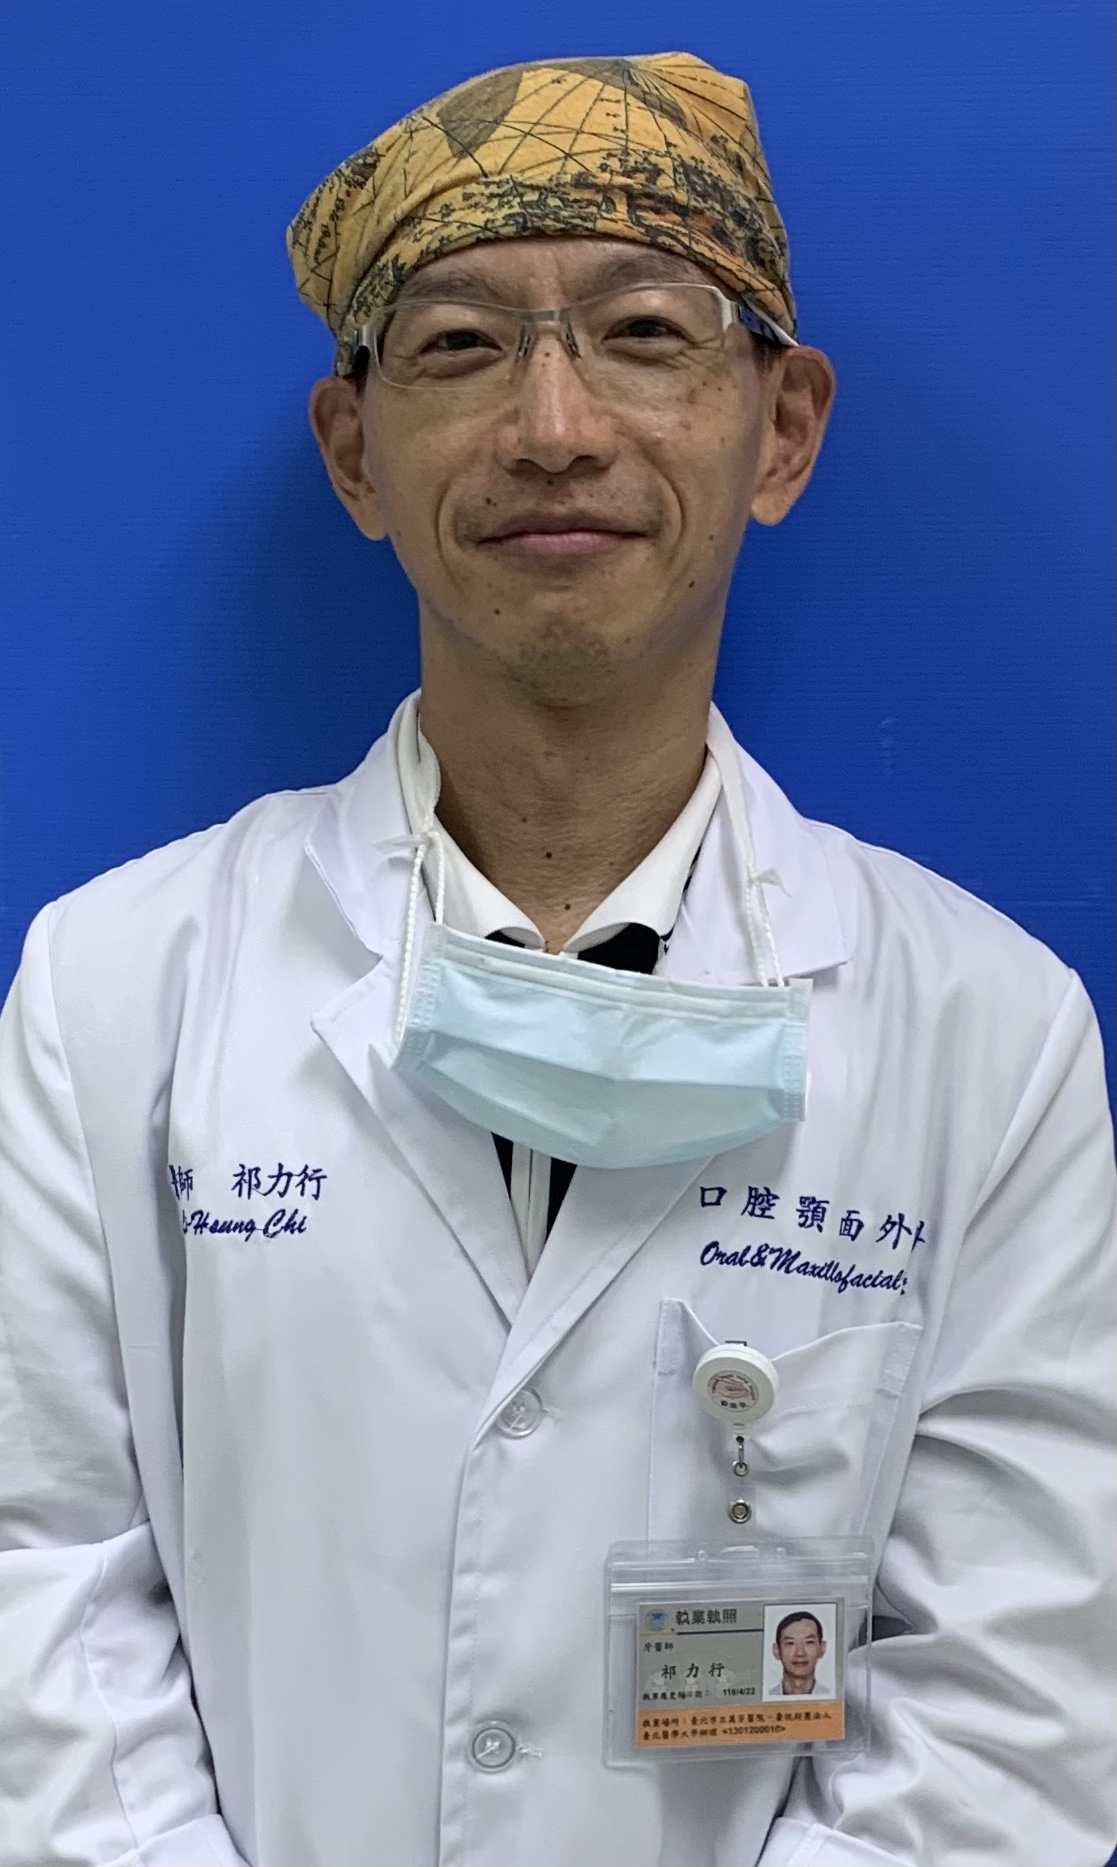
\includegraphics[height=6cm]{IMG_5507_Tex_portrait_TMWH.jpg}
\end{wrapfigure}

CURRICULUM VITAE

Tex, Li-Hsing Chi, D.D.S., Ph.D.\\
\noindent{Tel.: +886-970746815}\\
\noindent{E-mail: d622101005@tmu.edu.tw}

\begin{outline}

\0 Ph.D. candidate (since February, 2013--January, 2022):
\1 Prof. Michael Hsiao Lab\\
Genomics Research Center, Academia Sinica
\1 Prof. Yu-Chuan (Jack) Li Lab\\
Graduate Institute of Biomedical Informatics, College of Medical Science and Technology, Taipei Medical University
\0 Job: % Appointed: April, 2021--present
\1 Director, department of oral and maxillofacial surgery,
Wan Fang Hospital, Taipei Medical University (since April, 2021--present)

%\0 Job Appointed: January, 2003--present
\1 Attending physician and specialist, oral and maxillofacial surgery
Taipei Medical University Hospital, Taipei Medical University (since January, 2003--present)

\end{outline}



\paragraph*{Expertise and Research Interests}

My interests in research are i) to write the R/Python/C++ codes for biomedical data mining and deep learning of cancer research; ii) to establish the validation models of the genotype/phenotype changes \textit{\fontfamily{lmss}\selectfont in vitro} and \textit{\fontfamily{lmss}\selectfont in vivo}; iii) to develop molecular pathology and deep learning algorithm in the field of forensic medicine. 
As a well-trained physician-scientist, I could provide holistic patient care, deep learning science, and forensic medicine based on the findings of biomedical research.


\paragraph*{Qualifications}

B.S.---Sep. 1988 to Jun. 1994\\
Dental school, Taipei Medical University, Taipei, Taiwan

M.S.---Sep. 2011 to Jun. 2013\\
Biomedical Informatics, Taipei Medical University, Taipei, Taiwan

Ph.D. candidate---Feb. 2015 to Jan. 2022\\
\indent Ph.D.---Since Feb. 2022\\
The Ph.D. Program for Translational Medicine, College of Medical Science and Technology, Taipei Medical University and Academia Sinica, Taipei, Taiwan

\pagebreak

\paragraph*{Professional Membership}

-The specialist of Taiwan Academy of Oral and Maxillofacial Surgery (2002 - present)

-The member of International Association of Oral and Maxillofacial Surgeons (IAOMS)(2005)

-The member of Biophysics Society of R.O.C. (2014 to present)

-The member of Taiwan Society for Mitochondrial Research and Medicine (TSMRM) (2014)

-The member of Taiwan Society for Integration of Chinese and Western Medicine (TSICWM) (since 2020)

-The member of Chinese Medical Association of Acupuncture (CMAA), Taiwan (since 2020)

\paragraph*{Honor and Award}
Best Paper Presentation Award - 3rd Prize, at the 4th Translational Medicine Program Retreat, 2017


\paragraph*{Oral Presentation}
\begin{outline}


\1 Chi LH, Li YH, Pemg BY. Recurrent ameloblastic carcinoma ex ameloblastoma of maxilla - A case report. ICOMS – 17th International Conference on Oral and Maxillofacial Surgery, 2005. Vienna, Austria.
\1 Chi LH, Mac Cheng, Ajit Kumar, Chiang IJ, Li Yu-Chuan (Jack). A Summary of International Partnership for Health Informatics Education. IPHIE2012 Master class training of Health Informatics, 2012. University Of Minnesota, Twin Cities, MN, U.S.A.
\1 Chi LH, Wu TH Alex, Li Yu-Chuan (Jack), Hsiao M. Glucose Transporter 4, encoded by gene SLC2A4, as a Prognostic Marker for Head and Neck Squamous Cell Carcinoma. The 1st Annual Retreat of the Translational Medicine Degree Program, Sep. 19, 2014. Taipei, Taiwan.
\1 Chi LH, Wu TH Alex, Li Yu-Chuan (Jack), Hsiao M. Global Proteomics-based Identification and Validation of Thymosin Beta-4 X-Linked as a Prognostic Marker for Head and Neck Squamous Cell Carcinoma. The 4th Translational Medicine Program Retreat, Sep. 6, 2017. Taipei, Taiwan.
\1 Chi LH, Wu TH Alex, Hsiao Michael, Li Yu-Chuan (Jack). A Transcriptomic Analysis of Head and Neck Squamous Cell Carcinomas for Prognostic Indications. The 8th Annual Academic Achievements Presentation of Translation Medicine Degree Program, Sep. 10, 2021. Taipei, Taiwan.
\end{outline}

\paragraph*{Poster Presentation}

-Chi LH, Wu Alex, Li Jack, Hsiao M. Silencing JARID1B Suppresses Oncogenicity, Stemness and Increases Radiation Sensitivity in Head and Neck Squamous Cell Carcinoma. The 2nd Annual Retreat of the Translational Medicine Degree Program, Sep. 4, 2015. Kaohsiung, Taiwan, ROC. 

\textbf{\\
Profile Details \\
Last Updated: \today}

\end{vita}